A visual SLAM framework provides the foundation for integrating different components within it. 
For example, A visual SLAM system consists of camera tracking, mapping, loop closing, and visualization components. The framework connects the components such that we get the camera motion and the structure of the environment from a stream of images in real-time.


\section{Problem}

The outcome of this document is twofold: 
First, we want to find a \textit{good} way to connect the visual SLAM components. 
Second, while achieving the first outcome, we also define the structure of a repository in which the code is stored.
As a general rule of thumb, the \textit{good}ness of the framework is prioritized on the ease-of-use while maintaining the real-time capability.
Specifically, each component in the framework can be defined as a module, which can be customized or replaced for enhanced performance, so long as the interface (the inputs and outputs) is unchanged.

\section{Literature review}

A good visual SLAM framework allows for integrating the camera tracking, mapping, loop closing and visualization components and the intercommunication between them.
A good starting point is to study the self-driving car or autopilot projects on GitHub, notably \href{https://github.com/ApolloAuto/apollo}{Apollo by Baidu} and \href{https://gitlab.com/autowarefoundation/autoware.auto/AutowareAuto}{Autoware.Auto}\footnote{New versions of Autoware are under development, which can be found \href{https://github.com/autowarefoundation/autoware}{here}}.
They use their own middleware (\href{https://cyber-rt.readthedocs.io/en/latest/index.html}{Cyber RT}) and \href{https://docs.ros.org/en/humble/}{ROS2}. 
Wu et al.~\cite{wu2021oops} show that ROS2 is better than Cyber RT in terms of latency and CPU usage and recommend the use of shared memory (specifically intra-process (IAP) in ROS2) over data serialization/deserialization for the best latency and reliability.
Additionally, ROS2 is commonly adopted in robotics projects, with the support of new sensor integration. 

Among the existing visual SLAM systems, ORB-SLAM3 is one of the most practical and open-source visual SLAM system.
The practicality comes from the well-engineered algorithms designed to handle edge cases like improved camera tracking through multi-map merging and robust loop closure detection.

\section{Discussion}
To promote flexibility, we can organize the visual SLAM components as individual modules/libraries so that we can test them in isolation before integrating into the framework. As

\begin{figure}[h]
    \centering
    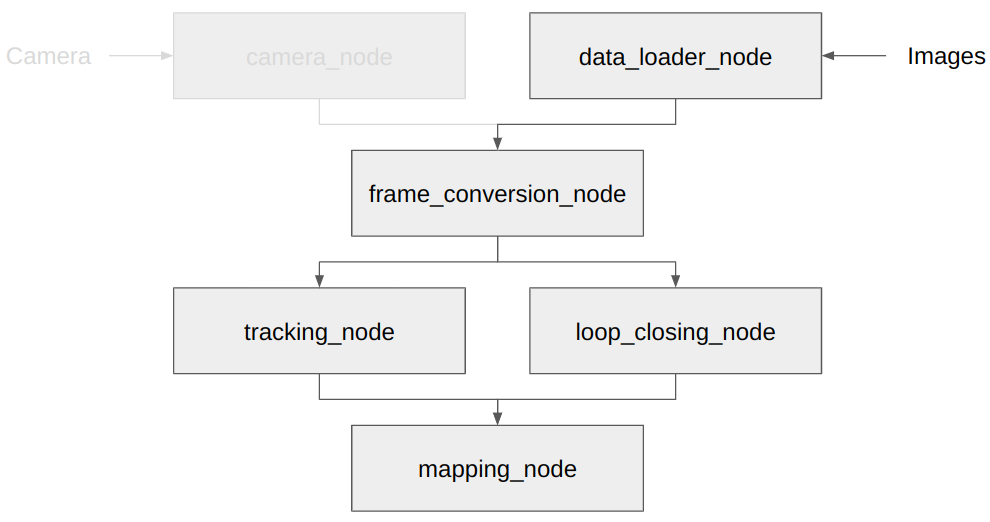
\includegraphics[width=0.5\textwidth]{img/pipeline.png}
    \caption{Visual SLAM pipeline}
    \label{fig:vslam_pipeline}
\end{figure}

Figure~\ref{fig:vslam_pipeline} shows the proposed visual SLAM pipeline with the components implemented as individual composable nodes. 
The role of each node is described as follows:
\begin{itemize}
  \item \textbf{data\_loader\_node} takes in a list of images from a folder and converts them into the Frame message, which contains the image and the camera information.
  
  \item \textbf{feature\_extraction\_node} calculates the features (e.g., corners or high-gradient image regions) in the image.
  
  \item \textbf{feature\_matching\_node} finds feature correspondences between the current frame and the nearest keyframe in the back-end during the tracking state.
  If the system is in the initialization state, the current frame will be set as the tentative keyframe and the node sets the mode to attempt initialization.
  In the attempt initialization state, any failure that occurs in tracking and mapping will reset the state back to initialization.
  If the system is in the relocalization mode, the current keyframe image is published to the place recognition node to find a candidate keyframe index, which is used to request the keyframe in the back-end to perform feature matching.
  In the event of failure to find correspondences, the node will set the state to relocalization.

  \item \textbf{tracking\_node} calculates the relative pose between the current frame and the current keyframe. 
  If the calculation fails to converge, then the node will set the state to relocalization. 

  \item \textbf{mapping\_node} triangulates a set of new map points based on the relative pose and the feature correspondences that don't have a 3D point. 

  \item \textbf{place\_recognition\_node} is used in two cases. 
  In the relocalization mode, it is used to find the candidate keyframe to recover tracking.
  When a new keyframe is created, it attempts to find a similar-looking image in the database and informs \textbf{feature\_matching\_node} to try to find new correspondences.

  \item \textbf{back\_end\_node} has two main responsibility: provide the current keyframe and optimize the graph based on the constraints given by the \textbf{feature\_matching\_node} and \textbf{tracking\_node}.
   
\end{itemize}

Note: after initialization, the current frame is added to the database in place\_recognition\_node for loop closure detection.

% Things to consider:
% https://design.ros2.org/articles/realtime_background.html
% https://arxiv.org/pdf/2101.02074.pdf

\subsection{Interfaces}


% * https://github.com/ZhenshengLee/ros2_shm_msgs/blob/humble/doc/Using_Zero_Copy_In_ROS2.pdf
% Octree to visualize millions of points? (https://github.com/heremaps/pptk)

\section{Appendix}

\subsection{Custom interfaces}

\subsubsection{Messages}

\begin{itemize}
  \item \textbf{vslam\_msgs/Frame}
  \begin{verbatim}
    # Header
    std_msgs/Header header

    # Camera information
    sensor_msgs/CameraInfo cam_info

    # Frame ID
    uint32 id 

    # Image
    sensor_msgs/Image image
    
    # Camera pose
    geometry_msgs/Pose pose
    
    # List of points
    vslam_msgs/Point [] pts
  \end{verbatim}

  \item \textbf{vslam\_msgs/FramePair}
  \begin{verbatim}
    # Constraint types
    uint8 FOR_INIT = 0
    uint8 FOR_TRACKING = 1
    uint8 FOR_LOOP_CLOSURE = 2
    uint8 FOR_RELOCALIZATION = 3

    # Constraints to be established in the feature matching and tracking 

    # The frame pair
    # frame1 is the existing/reference frame
    vslam_msgs/Frame frame1
    vslam_msgs/Frame frame2

    # Relative transformation
    geometry_msgs/Pose pose12

    # The matched points
    vslam_msgs/MatchedPoint [] matches

    uint8 constraint_type = 0
  \end{verbatim}

  \item \textbf{vslam\_msgs/MatchedPoint}
  \begin{verbatim}
    vslam_msgs/Point pt1    
    vslam_msgs/Point pt2
  \end{verbatim}

  \item \textbf{vslam\_msgs/Vector3d}
  \begin{verbatim}
    # unique point id for establishing correspondence
    uint64 id

    float64 x
    float64 y  
    float64 z 
  \end{verbatim}

  \item \textbf{vslam\_msgs/Vector2d}
  \begin{verbatim}
    # unique point id for establishing correspondence
    uint64 id

    float64 x 
    float64 y 
  \end{verbatim}

  \item \textbf{vslam\_msgs/Point}
  \begin{verbatim}
    uint32 frame_id
    
    # Keypoint
    vslam_msgs/Vector2d kp

    # Map point
    vslam_msgs/Vector3d mp
    bool has_mp = false
    
    # Feature
    vslam_msgs/Feature descriptor    
  \end{verbatim}

  \item \textbf{vslam\_msgs/Feature}
  \begin{verbatim}
    # The length and data structure of the descriptor to be 
    #   defined in the code
    uint32 len
    uint8 [] descriptor
  \end{verbatim}

  \item \textbf{vslam\_msgs/State}
  \begin{verbatim}
    uint8 INITIALIZATION = 0
    uint8 ATTEMPT_INITIALIZATION = 1
    uint8 TRACKING = 2
    uint8 RELOCALIZATION = 3
    
    uint8 state = 0
  \end{verbatim}
\end{itemize}

\subsubsection{Services}

\begin{itemize}
  \item \textbf{vslam\_msgs/GetKeyFrame}
  \begin{verbatim}
    # Get the keyframe with the provided frame id
    # Default to -1, which returns the current keyframe
    # In relocalization mode, place recognition node may 
    #   returns the frame id which can be used retrieve 
    #   the candidate keyframe for relocalization
    int64 frame_id = -1
    ---
    vslam_msgs/Frame keyframe
    
    # Return true if a keyframe is found
    bool has_keyframe
  \end{verbatim}

  \item \textbf{vslam\_msgs/SetKeyFrame}
  \begin{verbatim}
    # Assume nodes' good faith, i.e.,
    # nodes will not sabotage the system
    vslam_msgs/Frame keyframe
    ---
    # Indicate if the keyframe is set
    bool success
  \end{verbatim}

  \item \textbf{vslam\_msgs/FindKeyFrame}
  \begin{verbatim}
    # Attempt to find a similar-looking keyframe
    vslam_msgs/Frame frame
    ---
    # Indicate if a similar-looking frame is found
    # Default to -1, which means no similar-looking frame is found
    int64 frame_id = -1
  \end{verbatim}

  \item \textbf{vslam\_msgs/GetState}
  \begin{verbatim}
    ---
    # Get the state of the system 
    #   (e.g., initialization, tracking or relocalization)
    vslam_msgs/State state
  \end{verbatim}

  \item \textbf{vslam\_msgs/SetState}
  \begin{verbatim}
    # Set the state of the system 
    #   (e.g., initialization, tracking or relocalization)
    # Assume nodes' good faith, i.e.,
    # nodes will not sabotage the system
    vslam_msgs/State state
    ---
    # Indicate if the state is set
    bool success
  \end{verbatim}

  \item \textbf{vslam\_msgs/AddKeyFrameToDB}
  \begin{verbatim}
    # Add the frame to the database for loop closure detection
    vslam_msgs/Frame frame
    ---
    # Indicate if the frame is successfully added
    bool success
  \end{verbatim}
\end{itemize}

\subsubsection{Nodes}

\begin{itemize}
  \item \textbf{data\_loader\_node}
  \begin{itemize}
    \item Member functions:
\begin{lstlisting}
  # Publish the frame containing the image and camera information
  #   to @\textbf{frame\_callback}@
  @\textbf{publish\_frame}@()
\end{lstlisting}

    \item Member attributes:
\begin{lstlisting}
  # a folder containing the images
  Path @\textbf{path\_to\_images}@ 
    
  # A cam_info data structure containing the camera information 
  #   (e.g., intrinsics, distortion parameters, camera model, etc.)
  CamInfo @\textbf{cam\_info}@
\end{lstlisting}
  \end{itemize}  
  
  \item \textbf{feature\_extraction\_node}
  \begin{itemize}
    \item Member functions:
\begin{lstlisting}
  # Calculate the 2D features in the image
  # Algorithm:
  # image $\leftarrow$ get the image from the frame
  # Calculate the 2D feature points and, optionally, descriptors
  #   and save them in vslam_msgs/Point []
  # Publish vslam_msgs to @\textbf{frame\_matching\_callback}@
  @\textbf{frame\_callback}@(vslam_msgs/Frame) 

  # Private function:
  # Algorithm: 
  # Calculate and return a list of feature descriptors and their 
  #   keypoint location
  @\textbf{feature\_extractor}@(sensor_msgs/Image) $\rightarrow$ vector<vslam_msgs/Feature>
\end{lstlisting}

    \item Member attributes:
\begin{lstlisting}
  # A config data structure containing the feature extraction 
  #   settings (e.g., number of features)
  Config @\textbf{config}@
\end{lstlisting}
  \end{itemize}  


  \item \textbf{feature\_matching\_node}
  \begin{itemize}
    \item Member functions:
\begin{lstlisting}
  # Attempt to establish 3D-2D and/or 2D-2D correspondences
  # Algorithm:
  # state $\leftarrow$ Get the state from the back-end
  # if the state is INITIALIZATION
  #   set the current frame as the keyframe using 
  #     vslam_msgs/SetKeyFrame
  #   set the state as ATTEMPT_INITIALIZATION using 
  #     vslam_msgs/SetState
  # elif the state is ATTEMPT_INITIALIZATION or tracking
  #   curr_kf $\leftarrow$ Get the current keyframe
  #   matches $\leftarrow$ Find feature correspondences 
  #   if len(matches) < num_matches_thresh
  #     if state is ATTEMPT_INITIALIZATION
  #       Set the state to INITIALIZATION
  #     else
  #       Set the state to RELOCALIZATION
  #     return
  #   else
  #     frame_pair $\leftarrow$ Create a vslam_msgs/FramePair 
  #     populate the frame_pair attributes 
  #     if state is ATTEMPT_INITIALIZATION
  #       set constraint type in frame_pair to FOR_INIT
  #     else
  #       set constraint type in frame_pair to FOR_TRACKING
  #     publish frame_pair to @\textbf{frame\_tracking\_callback}@
  # else # the state is RELOCALIZATION
  #   candidate_frame_id $\leftarrow$ Find a candidate keyframe using
  #   candidate_keyframe $\leftarrow$ Get the candidate keyframe using the id
  #   matches $\leftarrow$ Find feature correspondences
  #   if len(matches) > num_matches_thresh:
  #     frame_pair $\leftarrow$ Create a vslam_msgs/FramePair 
  #     populate the frame_pair attributes 
  #     set constraint type in frame_pair to FOR_RELOCALIZATION
  #     publish frame_pair to @\textbf{frame\_tracking\_callback}@
  @\textbf{frame\_matching\_callback}@(vslam_msgs/Frame) 

  # Attempt to establish 3D-2D correspondences
  #   when a new keyframe is created and a candidate loop is found
  # Algorithm:
  # frame_id $\leftarrow$ Get frame1's id (the candidate keyframe)
  # frame1 $\leftarrow$ Get the frame using the frame_id from back-end
  # matches $\leftarrow$ Find feature correspondences
  # if len(matches) > num_matches_thresh:
  #   publish frame_pair to @\textbf{loop\_tracking\_callback}@
  @\textbf{loop\_matching\_callback}@(vslam_msgs/FramePair)
\end{lstlisting}

    \item Member attributes:
\begin{lstlisting}
  # Minimum number of matches
  @\textbf{num\_matches\_thresh}@
\end{lstlisting}
  \end{itemize}  

  \item \textbf{tracking\_node}
  \begin{itemize}
    \item Member functions:
\begin{lstlisting}
  # Calculate the relative transformation between the frame pair
  # Algorithm:
  # if constraint_type is FOR_INIT
  #   tracking_quality, pose12 $\rightarrow$ calculate the relative pose 
  #     from 2D-2D correspondences
  #   if tracking_quality is good
  #     publish frame_pair to @\textbf{mapping\_callback}@
  #   else
  #     set the state to RELOCALIZATION
  # elif constraint_type is FOR_TRACKING
  #   tracking_quality, pose12 $\rightarrow$ calculate the relative pose 
  #     from 3D-2D correspondences
  #   if tracking_quality is good
  #     Attempt to find a closed loop to establish another constraint
  #     frame_id $\rightarrow$ find a candidate keyframe
  #     if frame_id != -1:
  #       candidate_keyframe $\rightarrow$ get the candidate keyframe
  #       frame_pair $\rightarrow$ create a FramePair instance
  #       populate frame_pair with relevant information 
  #         (e.g., frame1=candidate_keyframe, frame2=current_frame)
  #       publish the frame_pair to @\textbf{place\_recognition\_callback}@
  #     
  #     if pose12 satisfies the new keyframe criteria
  #       add the current keyframe to the place_recognition_node  
  #         database using 
  #       publish the frame_pair to @\textbf{mapping\_callback}@
  #   else
  #     set the state to RELOCALIZATION
  @\textbf{frame\_tracking\_callback}@

  # Calculate the relative transformation of a potential loop 
  #   constraint
  # Algorithm:
  # # Mutual consistency check 
  # get frame1 and frame 2 from frame_pair
  # tracking_quality1, pose12 $\rightarrow$ calculate the 3D-2D camera pose from 
  #   frame1 to frame2
  # tracking_quality2, pose21 $\rightarrow$ calculate the 3D-2D camera pose from 
  #   frame2 to frame1
  # if both tracking_quality1 and tracking_quality2 are good
  #   if pose12 * pose21 is small
  #     set pose12 in frame_FramePair
  #     publish frame_pair to @\textbf{loop\_constraint\_callback}@
  @\textbf{loop\_tracking\_callback}@(vslam_msgs/FramePair)

  # Private function
  # Calculate 3D-2D camera pose
  @\textbf{track\_camera\_3d2d}@

  # Private function
  # Calculate 2D-2D camera pose
  @\textbf{track\_camera\_2d2d}@
\end{lstlisting}

    \item Member attributes:
\begin{lstlisting}

\end{lstlisting}
  \end{itemize} 

  \item \textbf{mapping\_node}
  \begin{itemize}
    \item Member functions:
\begin{lstlisting}
  # Triangulate new map points based on the matched 2D-2D 
  #   correspondences
  # Algorithm:
  # frame_pair $\rightarrow$ FramePair msg
  # Iterate through the matched points:
  #   if there is no 3D point:
  #     pt_3d $\rightarrow$ Triangulate the point based on the pose and match
  #     pt->mp = pt_3d
  # publish the frame_pair to @\textbf{frame\_constraint\_callback}@
  @\textbf{mapping\_callback}@(vslam_msgs/FramePair)
  
\end{lstlisting}

    \item Member attributes:
\begin{lstlisting}

\end{lstlisting}
  \end{itemize} 

  \item \textbf{place\_recognition\_node}
  \begin{itemize}
    \item Member functions:
\begin{lstlisting}
  # Find the candidate keyframe
  # Algorithm:
  # Calculate the similarity score of the frame against the database
  # if a similar frame is found
  #   frame_pair <- Create a frame_pair object
  #   set frame1's ID in the frame_pair as the frame found in 
  #     database
  #   set frame2 as the incoming frame
  #   publish frame_pair to @\textbf{loop\_matching\_callback}@
  @\textbf{place\_recognition\_callback}@(vslam_msgs/Frame)
  
  # Find keyframe service callback
  @\textbf{find\_keyframe\_srv\_callback}@(vslam_msgs/FindKeyFrame)

  # Add keyframe to database service callback
  @\textbf{add\_keyframe\_srv\_callback}@(vslam_msgs/AddKeyFrameToDB)
\end{lstlisting}

    \item Member attributes:
\begin{lstlisting}

\end{lstlisting} 
  \end{itemize} 
  \item \textbf{back\_end\_node}
  \begin{itemize}
    \item Member functions:
\begin{lstlisting}
  # Is used when a new keyframe is inserted
  # Algorithm:
  # push the frame constraint to the constraints queue
  @\textbf{frame\_constraint\_callback}@(vslam_msgs/FramePair)

  # Is used when a loop constraint is found
  # Algorithm:
  # push the loop constraint to the constraints queue
  @\textbf{loop\_constraint\_callback}@(vslam_msgs/FramePair)

  # Get keyframe service callback
  @\textbf{get\_keyframe\_srv\_callback}@(vslam_msgs/GetKeyFrame)

  # Set keyframe service callback
  @\textbf{set\_keyframe\_srv\_callback}@(vslam_msgs/SetKeyFrame)

  # Get state service callback
  @\textbf{get\_state\_srv\_callback}@(vslam_msgs/GetState)

  # Set state service callback
  @\textbf{set\_state\_srv\_callback}@(vslam_msgs/SetState)

  # Private function
  # Algorithm:
  # constraint $\leftarrow$ pop one constraint from the constraints queue
  # if constraint type is FOR_TRACKING
  #   run local bundle adjustment
  # elif constraint type is FOR_LOOP_CLOSURE
  #   run graph optimization
  @\textbf{optimization\_loop}@()
\end{lstlisting}

    \item Member attributes:
\begin{lstlisting}
  # Queue for adding frame and loop constraints
  queue<vslam_msgs/FramePair> constraints

  # An ordered map for quick look-up
  map<int64, vslam_msgs/Frame> frames

  # State
  vslam_msgs/State state
  
  # Current keyframe
  vslam_msgs/Frame current_kf

  # Internally managed graph
  # To be modified by the provided constraints in the constraints 
  #   queue
  map<vslam_msgs/Frame, vector<Constraint3D2D>> constraints_3d2d 
  map<vslam_msgs/Frame, vector<ConstraintPose>> constraints_pose
\end{lstlisting}
  \end{itemize} 
\end{itemize}

\subsection{ROS2 study}

To ensure ROS2 is the right fit for the visual SLAM framework, we need to experiment with the modularity and the memory-sharing mechanism provided by it.
\href{https://github.com/ros-planning/navigation2}{Nav2} provides examples of creating action servers (e.g., planner and controller), each of which could have several plugins to accomplish various tasks.
The action servers are ROS2 nodes managed by their \href{https://github.com/ros2/demos/blob/humble/lifecycle/README.rst}{lifecycle manager} to activate or deactivate the nodes on demand.
The nodes are loaded as \href{https://docs.ros.org/en/humble/How-To-Guides/Launching-composable-nodes.html}{composable nodes} to allow for \href{https://docs.ros.org/en/humble/Tutorials/Demos/Intra-Process-Communication.html}{intra-communication} among the nodes.
Therefore, we could use action servers to represent the core components in the visual SLAM system and potentially use intra-process communication to reduce the overhead from unnecessary data copy between nodes.
